\documentclass{article}
\usepackage[margin=1in]{geometry}
\usepackage{amsmath,amsthm,amssymb}
\usepackage{bbm,enumerate,mathtools}
\usepackage{tikz,pgfplots}
\usepackage{chessboard}
\usepackage[hidelinks]{hyperref}
\usepackage{multicol} % Problem 35

\newenvironment{question}{\begin{trivlist}\item[\textbf{Question.}]}{\end{trivlist}}
\newenvironment{note}{\begin{trivlist}\item[\textbf{Note.}]}{\end{trivlist}}
\newenvironment{references}{\begin{trivlist}\item[\textbf{References.}]}{\end{trivlist}}
\newenvironment{related}{\begin{trivlist}\item[\textbf{Related.}]\end{trivlist}\begin{enumerate}}{\end{enumerate}}


\begin{document}
\rating{2}{2}
The puzzle Figure/Ground by Ian Gilman features a grid with two colors. In the
grid any (horizontal/vertical) connected component can be moved exposing the
other color beneath.
\begin{figure}[ht!]
  \centering
  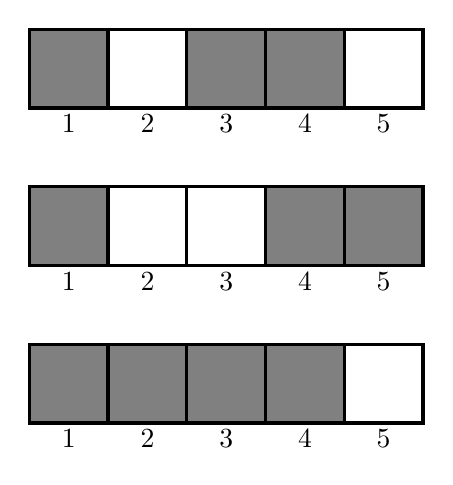
\begin{tikzpicture}
    \foreach \i/\c in {1/gray, 2/white, 3/gray, 4/gray, 5/white} {
      \draw[very thick, fill=\c] (\i, 0) rectangle (\i + 1, 1);
      \node at (\i + 0.5,-0.2) {\i};
    }

    \foreach \i/\c in {1/gray, 2/white, 3/white, 4/gray, 5/gray} {
      \draw[very thick, fill=\c] (\i, -2) rectangle (\i + 1, -1);
      \node at (\i + 0.5,-2.2) {\i};
    }

    \foreach \i/\c in {1/gray, 2/gray, 3/gray, 4/gray, 5/white} {
      \draw[very thick, fill=\c] (\i, -4) rectangle (\i + 1, -3);
      \node at (\i + 0.5,-4.2) {\i};
    }
  \end{tikzpicture}
  \caption{
    It is possible to get from the first configuration to the second
    configuration by moving the $(3,4)$-block to position $(4,5)$ or by moving
    the $5$-block to position $3$.
    It is possible to get from the first configuration to the third by moving
    the block in position $2$ to position $5$.
  }
\end{figure}

\begin{question}
  Is there an efficient algorithm to determine whether it's possible to get from
  one configuration to another?
\end{question}

\begin{related}
  \item On a $1 \times n$ grid, what is the greatest number of steps between two
  configurations?
  \item Starting with the $1 \times n$ grid where even squares are black and
  odd squares are white, is is possible to get to any configuration with both
  colors present? Do other starting configurations have this property?
  \item What if this is done on a $n \times m$ grid?
  A $n_1 \times \hdots \times n_k$ grid?
  A triangular/hexagonal grid? Torus?
  \item What if more colors were used?
\end{related}


\begin{references}
  \item \url{http://www.clockworkgoldfish.com/figureground/list/sky/}
\end{references}

\end{document}
